\section{Evaluation}
 At this time, we are not aware of any available "gold standard" dataset for hashtag meanings.  In order to compensate, we were forced to create our own test dataset, which consisted of a spreadsheet with 27 hashtags, and known relevant links to each of those hashtags. We understand that this is a small dataset, and not statistically significant, thus is a weak point of our system. We did, in addition, do many heuristic based tests to see if we were getting relevant results based on the links that the system returned. We observed that in addition to noisy results, the system did often return at least one or two of the most relevant documents to a particular hashtag. The text summarization aspect did not perform very well, and we attribute this to the fact that in order to generate an accurate summary, the top few links returned must be very relevant to the hashtag, otherwise it will be a completely inaccurate summary.\\
 
 
 \begin{figure}[h!]
     \fbox{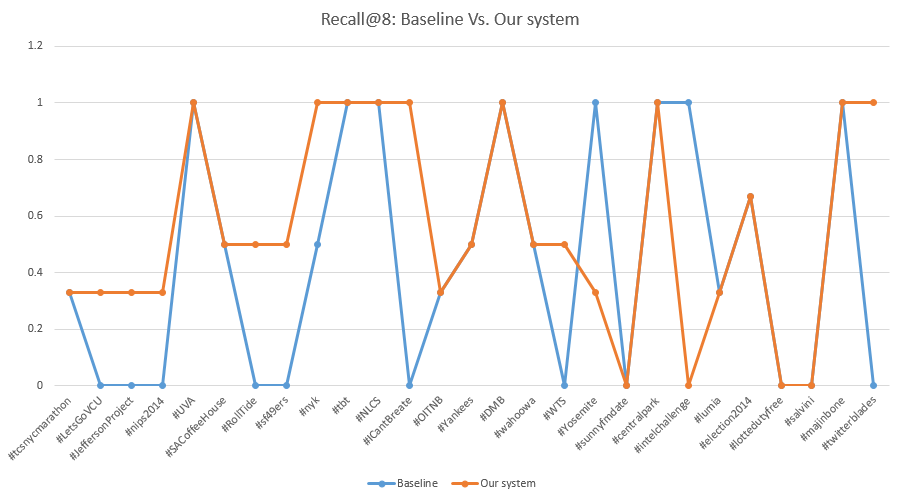
\includegraphics[width=.46\textwidth]{recallat8}}
   \caption{Evaluation results} \label{fig:recallat8}
\end{figure}



\begin{table}[h]
    \centering
    \caption[Table caption text]{Average recall@8.}
    \label{table:recall}
    \begin{tabular}{ | l | l | l |} \hline
    & Baseline & Our system \\ \hline
    Ave. recall@8 & 0.43 & 0.55 \\ \hline
    Matched Hashtags & 16/27 & 23/27 \\ \hline
    \end{tabular}
    
\end{table}